\documentclass[jou,apacite]{apa6}   %Utilizamos Apa6 mas actualizada, de tipo jorunal.

\usepackage[utf8]{inputenc}       	%Encoding de Utf-8, por compatibilidad con mi vim.
\usepackage[T1]{fontenc}			%Determina que tipo de fuente sera usado
\usepackage[spanish]{babel}			%Idioma manejado para el articulo
\usepackage{subfigure} 				%Subfiguras
\usepackage{graphicx}				%Necesario para el manejo de imagenes en el articulo.
\DeclareGraphicsExtensions{.png,.jpg,.jpeg}%Extensiones Soportadas para las imagenes.

%Las imagenes se encuentran en directorio de /images/, mas info en https://en.wikibooks.org/wiki/LaTeX/Importing_Graphics

\title{Descubriendo Controladores Lógicos Programables en una Red Universitaria} 
\shorttitle{ Descubriendo PLC's en una Red Universitaria}
\twoauthors{Héctor Fabio Jiménez Saldarriaga}{Sebastian Zapata Ruiz}
\twoaffiliations{Universidad Tecnológica de Pereira, \\ Ingeniería de Sistemas y Computación, \\Pereira Security Team }{Universidad Tecnológica de Pereira, \\ Ingeniería de Sistemas y Computación}
\keywords{Redes Industriales , Seguridad Informática, Controladores Lógicos}
\abstract{El uso de los dispositivos electrónicos como los controladores lógicos programables  en el campo de la automatización y el control de procesos tienen un rol importante, estos se implementan en muchos campos, e industrias donde los procesos de producción y  administración son complicados,  críticos y peligrosos tanto económicamente como para la vida humana.  En este artículo evidenciamos cómo es posible realizar el descubrimiento de estos dispositivos en un entorno controlado que presenta múltiples PLC's, Computadores de Monitoreo corriendo bajo sistemas operativos Windows, en un	a infraestructura universitaria.}
\leftheader{Héctor F. Jiménez S., Sebastian Zapata R.} %Header en la parte superior.

\begin{document}
\maketitle    
                     
\section{Introducción}
Los controladores lógicos programables (\textit{Programmable logic controller}, de ahora en adelante PLC) fueron diseños en los años 60s[Ref1, Segovia]
cuando el control de las maquinas industriales se hacía mediante el uso de relés como en la figura (\ref{fig:cuartoreles}), en ese entonces era tedioso
y complicado para un técnico encontrar una falla en el sistema eléctrico de control debido a que todo los procesos se encontraban en cuartos llenos de  
una gran cantidad de cables y relés, lo que dificultaba la búsqueda. Con la llegada de los  PLCs se resolvió el problema de la flexibilidad y solución 
de problemas comunes; estos reemplazaron decenas de cuartos en pocos, albergando bloques compactos de PLC, con ventajas como fácil mantenimiento,
instalación, expansión. Su labor principal es la regulación  los actuadores electromecánicos, como pueden ser válvulas, sensores, bombas, motores, etc.\\

\begin{figure}[htb]
\centering
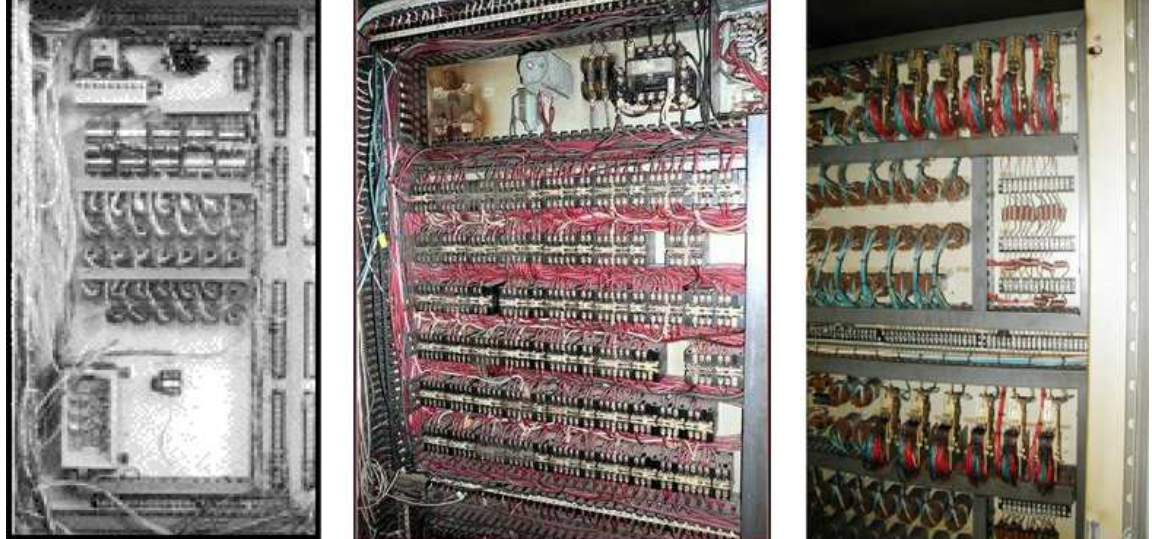
\includegraphics[scale=0.28]{images/relayroom.png}
\caption{Cuarto de Control Reles, 1974.} \label{fig:cuartoreles}
\end{figure}

Los sistemas de control utilizan como uno de los elementos conformantes  a los PLCs  para regular procesos industriales  ejemplos de estas tareas se ve
en lineas de producción de químicos, líneas de ensamble y manufactura, maniobra de maquinaria pesada,  control y manejo de señales, control de mezclas, 
control de generación y despacho eléctrico entre otros(Referencia Porcentajes). En un principio de estos dispositivos se presentaba la situación de que 
cada PLC actúa como controlador individual e independiente, pero con el crecimiento y demanda de los procesos se requería tener conexiones con otros 
PLCs, pero funcionando aun así en un contexto local, sin conexiones a redes corporativas o Internet(Ref ENISA, Protecting Industrial Control Systems). 
En los últimos 15 años con la globalización y la descentralización de las empresas que administran estos procesos se vuelve necesario tener que 
conectar estos dispositivos mediante enlaces privados e infraestructura pública, sin tener en mente los pilares de la seguridad de la información, 
confidencialidad, integridad, autenticidad.\\


Una parte esencial de los sistemas de control industrial (de ahora en adelante SCI) son los sistemas SCADA (\textit{Supervisory Control and Data Acquisition}), responsables de obtener información relevante y basados en el análisis de esta información enviar instrucciones a los sistemas de producción. Los sistemas SCADA necesitan estar conectados en varias niveles topológicos dentro del sistema de control industrial,  ejemplo de ello se puede ver en la figura (\ref{fig:sci}). 
\section{Sistemas de Control Industrial (SCI)}
Un sistema de Control industrial se compone de distintos elementos y zonas como se muestra en la figura(\ref{fig:sci}),  los más representativos son :
\begin{itemize}
  \item Sistema de administración de  operaciones
  \item Gestión de operaciones Comerciales
  \item Sistema de Control y Adquisición de Datos
  \item Red de Supervisión
  \item Sistemas de Proceso y Control \ldots
\end{itemize}

\begin{figure}[htb]
\centering
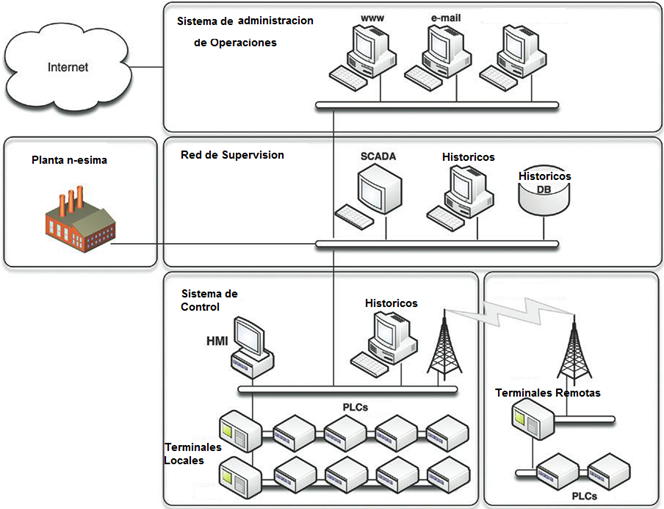
\includegraphics[scale=0.5]{images/sci.png}
\caption{Sistemas de Control Industrial (SCI)} \label{fig:sci}
\end{figure}
Cada zona o elemento tiene su propio fin físico y lógico, además de las consideraciones de seguridad, y políticas a implementar, se debe de ver que  existen dependencias entre los diferentes niveles. 

\subsection{Sistema SCADA y Protocolos }
Un sistema SCADA típico consiste de diferentes partes. El algoritmo de control de más bajo nivel se ejecuta en un PLC o terminal remota. Estos dispositivos están conectados a sensores y actuadores. Ellos reciben los datos proporcionados por los sensores, evalúan el estado del sistema local  y controlan los actuadores basados en el resultado del análisis de los datos. Los PLC pueden ser conectados en diferentes topologías e integrarse entre sí para ser supervisados y monitoreados por el SCADA como se muestra en la pirámide de automatización 
\begin{figure}[htb]
\centering
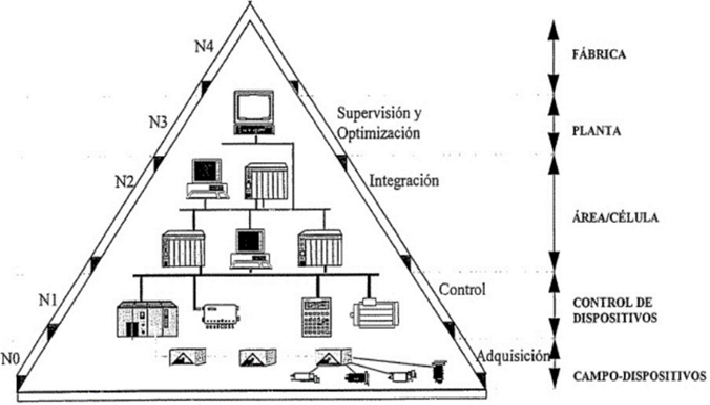
\includegraphics[scale=0.4]{images/piramide.png}
\caption{Piramide de Automatización,Niveles.} \label{fig:piramide}
\end{figure}
Para alcanzar el Sistema de supervisión se requiere de una computadora normal típicamente corriendo alguna versión de software SCADA  [ListofScadaRef] que permite realizar diagnósticos remotos, envió de instrucciones o reprogramación de control a los PLCs. Una base de datos de históricos almacena datos de los eventos presentados  en el pasado para evaluaciones futuras [RefTrendMicro]. 

Los SCADA hacen uso de protocolos de redes estandar para el transporte de administración y  programación de los comandos del PLC. Los protocolos también se utilizan para la comunicar entre PLCs. La conexión a las redes corporativas o Internet. Por ejemplo, para el \textit{mantenimiento remoto}: se realiza con frecuencia a través de protocolo estándar, como HTTP, Telnet o FTP. Conectividad en la capa de enlace que por lo general se lleva a cabo a través de Ethernet.

Los protocolos mas usados para los sistemas SCADA son DNP3, ICCP (IEC 60870-6), Modbus, OPC (OLE for process control), Profibus,CIP, cada uno de estos posee distintas características y sistemas de seguridad, cifrado, aun así, cada uno posee diferentes vulnerabilidades a posibles ataques e inclusive algunos de ellos no realizan ninguna comprobación de seguridad.

\subsection{Problemas Generales de Seguridad en un SCI }
Mencionar uno de las preguntas del nuestra investigación entorno a un SCI.

\section{Configuración del Análisis de Seguridad}
Para el desarrollo de esta investigación seguiremos una metodología de seguridad como OSSTMM, además las propuestas prácticas de Dale Peterson(Referencia), Robert Graham, Paul Mcmillan, Dan Tencler (Referencia), y por supuesto recomendaciones del equipo de Zmap https://zmap.io/documentation.html\#bestpractices).

Es importante aclarar que el posicionamiento que se tomo es  interno, con una visibilidad blackbox esto significa que no contamos con ninguna inforamcion del objetivo, pero los dueños de la red tienen conocimientode que tipo de pruebas se realizara y cuando. Se adoptao un perfil de usuario normal, sin privilegios, hay que mencionar que nosotros obtuvimos los permisos legales para  llevar a cabo esta investigación pues es de realizar estas actividades sin el permiso correspondiente,  podría incurrir en algún acto tipificado como delito informático. El proceso se realizó en un entorno controlado(RefEntControlado) que implico solamente el escaneo de  algunas subredes de nuestra red universitaria, desconociendo la topología de la red como se menciono previamente. Se utilizo un computador portátil, y un mini servidor de escritorio ambos corriendo Debian Gnu/Linux, con procesadores Core2Duo, 2xCore I7,  4 y 8 Gb  de Ram, con tarjetas 100/1000, dual-port, conectados a la red que tienen acceso normalmente los estudiantes.

En el escaneo de puertos se emplearon las tres herramientas más populares que son:
\begin{itemize}
\item Zmap: Desarrollado por un equipo de tres científicos de computación en la universidad de Michigan, ellos son Ph.D  Akir Durumeric, Ph.D(c) Eric Wustrow, y J. Alex Halderman, Profesor asistente, el software se encuentra bajo la licencia de Apache Foundations.
\item Masscan: Desarrollado por Robert David Graham el escáner de puertos más rápido del momento, que requiere de un computador con un procesador de 4 núcleos y una tarjeta ethernet dual-port de 10gbs, teóricamente puede transmitir 25 millones de paquetes por segundo, aunque en nuestras pruebas solo utilizamos 8 millones de paqueter por segundo para no congestionar y perjudicar la red, este software se encuentra licenciado bajo Gnu Gpl v3.
\item Nmap: El scanner que más utilizamos en nuestra fase de reconocimiento activo,  es una herramienta de código abierto para exploración de red y auditoria de seguridad. Su líder de desarrollo es Fyodor, este escáner tiene una gran importancia en nuestra investigación puesto que posee un motor de scripting en el cual cargamos los scripts desarrollados por Digitalbond(Ref) una compañía que se encarga de asegurar sistemas y redes industriales.
\end{itemize}
El escaneo indica el estado de los puertos de las máquinas, dispositivos conectados a las redes, detectando y descubriendo si está abierto, cerrado, o protegido por un  cortafuegos. Esto nos puede indicar que tipo de servicio ofrece, y por lo tanto poder determinar la exposición de equipos vulnerables. La siguiente imagen presenta una topología aproximada, basados en los datos arrojados por las herramientas, y cantidad de saltos mostrados mediante tracert.
\begin{figure}[htb]
\centering
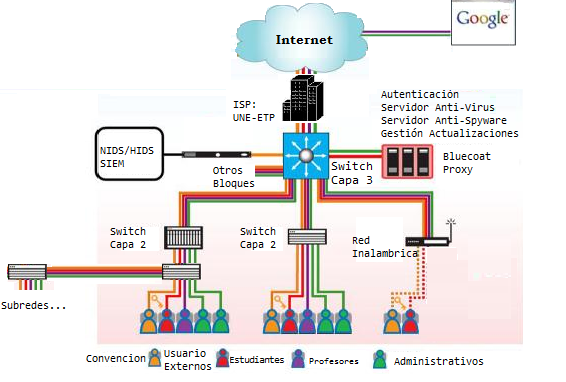
\includegraphics[scale=0.6]{images/topologia.png}
\caption{Topologia aproximada, posicionamiento interno.} \label{fig:topologiared}
\end{figure}
\section{Posibles Ataques}
Según el protocolo que usen los sistemas SCADA,PLCs pueden poseer distintas vulnerabilidades, algunos de estos poseen comprobaciones de seguridad, pero aun así las tienen, por ejemplo el protocolo Modbus, cuyo diseño está pensado para operar sobre líneas de transmisión en serie. El modo bajo el cual se da la comunicación de estas redes es un primitivo esquema de “petición-respuesta”, que dificulta la identificación de un eventual ataque pues los sistemas no podrían distinguir entre peticiones legítimas o peticiones provenientes de sistemas infectados. El protocolo Modbus está montado sobre TCP y ese protocolo no realiza autenticación ni tiene funcionalidades de confidencialidad de manera nativa, de forma tal que una vez que el atacante logra entrar a la red puede tomar el control de una sesión y comprometer los dispositivos o alterar datos del SCADA.

Ataques comunes a los PLCs o también llamados Stuxnet son gusanos que afectan a equipos con Windows, descubierto en junio de 2010 por VirusBlokAda, una empresa de seguridad radicada en Bielorrusia. Es el primer gusano conocido que espía y reprograma sistemas de control industrial, en concreto sistemas SCADA de control y monitorización de procesos, llegando a afectar las infraestructuras críticas como centrales nucleares.
Cuando Stuxnet fue descubierto tenia capacidades de reprogramacion de controladores lógicos programables y ocultar los cambios realizados. 
Algunos Otros posibles ataques a los sistemas SCADA:
\begin{itemize}
\item DoS, es un ataque a la denegación de servicios, causa que un servicio o recurso sea inaccesible a los usuarios legítimos. Normalmente provoca la pérdida de la conectividad de la red por el consumo del ancho de banda de la misma.
\item Spoofing, el atacante se hace pasar por una entidad distinta a través de la falsificación de los datos en una comunicación.
\item 
\item 
\end{itemize}

\section{Resultados }
Durante el análisis realizado a las \textbf{8192} direcciones IP utilizando los escáneres Zmap, Masscan y Nmap se utilizaron para  correlacionar la información, se utilizó la lista de puertos de PLCs más probables que podrían ser utilizados en el país como son las compañías
\begin{enumerate}
\item Allen Bradley,
\item Zilog
\item Siemens
\item Hagger
\end{enumerate}

El experimento se realizó en los segmentos de red de los edificios de \textit{eléctrica, bloque administrativo, y edificio de sistemas} donde se detectó que no se implementan políticas y reglas adecuadas en los sistemas de detección de intrusos(\textit{HIDS,NIDS}) lo cual fue notificado a los administradores de la red para tomar las medidas correspondientes, pues se generó una gran cantidad de paquetes que podrían haber detenido y afectado directamente los dispositivos de red como switches y routers por la cantidad de trafico entrante. Se pudo observar también que las redes virtuales inalámbricas se encuentran bien segmentadas pues no fue posible acceder a otros segmentes de red a través de estas.El cuadro (\ref{prueba}).  presenta un resumen conciso de lo hallado.

\begin{table}[htb]
\centering
\begin{tabular}{| p{1.8cm}| p{1.1cm} |p{1.9cm}|p{1.2cm}|}
\hline
\multicolumn{4}{|c|}{Estadísticas de Detección} \\
\hline
Marca & Puerto & Segmento & Cantidad\\
\hline 
Siemens & 103 & Eléctrica & 6\\ \hline
AllenBradley & num  & Administrativo & 4\\ \hline
Zilog y Otros & num  & Sistemas y Eléctrica & 3 \\ \hline
\end{tabular}
\caption{Resultados Obtenidos, Nmap, Zmap, Masscan.}
\label{fig:prueba}
\end{table}
Despues de obtener los datos por segmentos ubicamos algunos de ellos detectando que muchos de ellos son utilizados para prácticas de laboratorios como en las figuras  (\ref{fig:s7200}),(\ref{fig:s73002}),(\ref{fig:simulacion}).

\begin{figure}[htb]
\centering
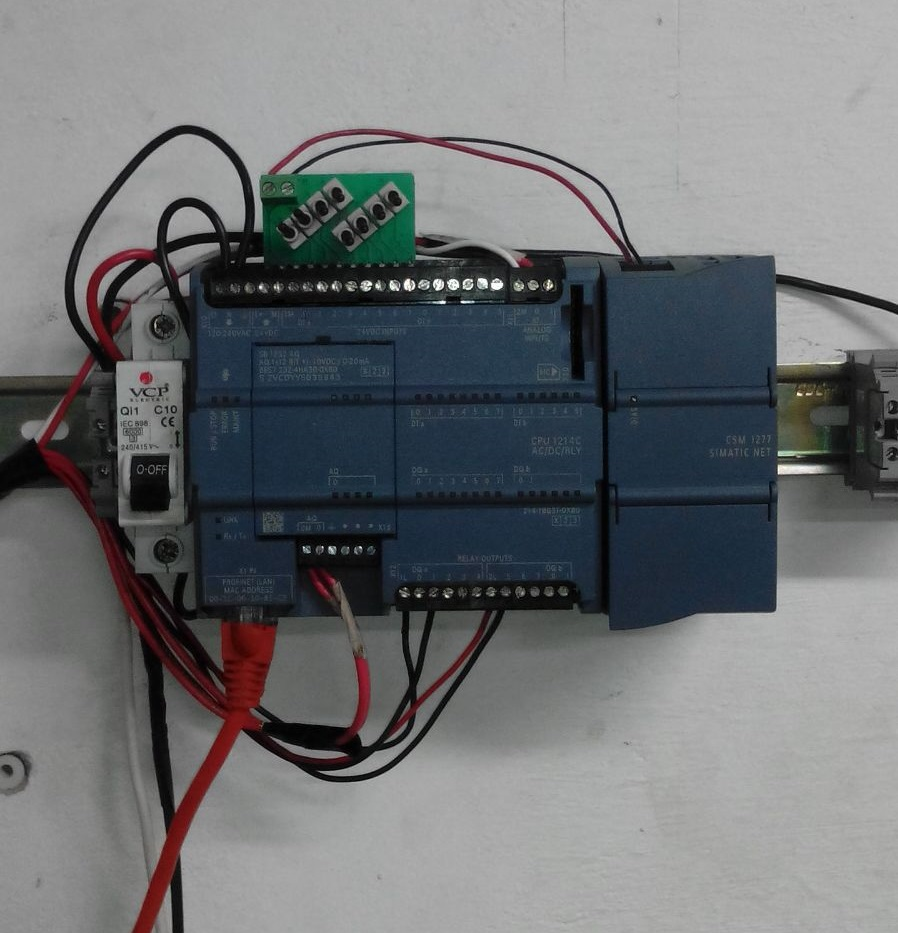
\includegraphics[scale=0.2]{images/s71200.jpg}
\caption{Siemens S7-1200,Red Profinet. Control de Banco Hidraulico.} \label{fig:s7200}
\end{figure}
Algunos de las practicas se encontraban funcionando, si hubiéramos tomado una posición ofensiva hubiera sido posible ocasionar daños materiales, y humanos a los estudiantes dentro del laboratorio.
\begin{figure}[htb]
\centering
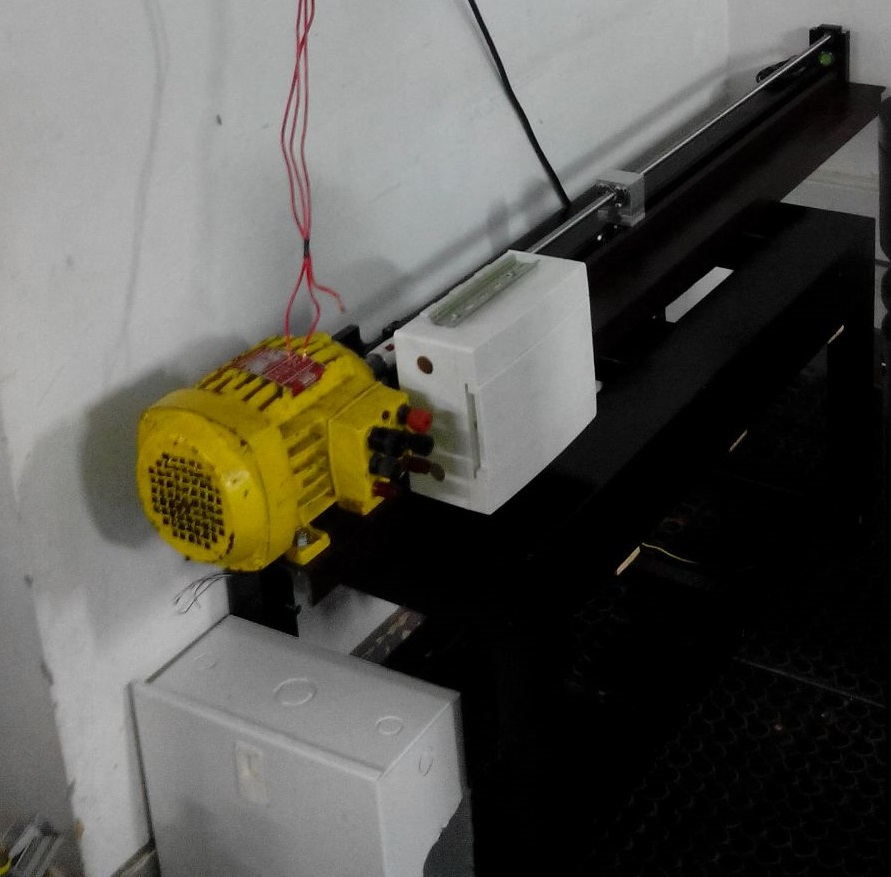
\includegraphics[scale=0.2]{images/motorsimulacion.jpg}
\caption{Motor de 3hp, Control de Velocidad posicionamiento de tornillo, practica realizada por estudiantes mediante controladores logicos programables.} \label{fig:simulacion}
\end{figure}

\begin{figure}[htb]
\centering
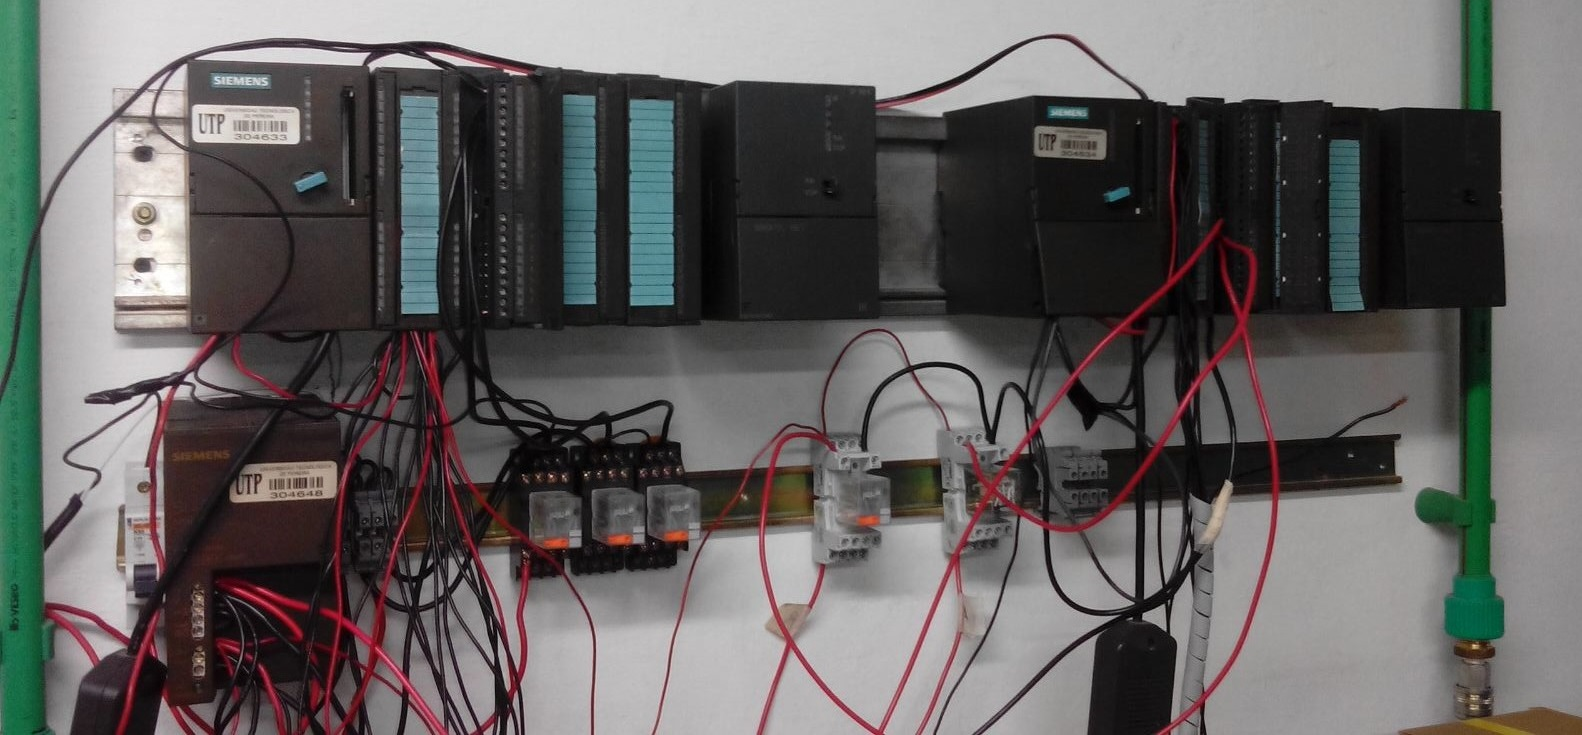
\includegraphics[scale=0.2]{images/s73002.jpg}
\caption{Siemens S7-300, Red Profibus-Profinet} \label{fig:s73002}
\end{figure}
\newpage
\section{Conclusiones }
En conclusión es posible hallar y descubrir dispositivos que regulan procesos críticos dentro de una red universitaria, se deben utilizar y aplicar las políticas y medidas de seguridad al respecto a este tipo de dispositivos y sistemas, pues estos dispositivos están constantemente conectados a la red de forma continua presentando riesgo de alto impacto para los estudiantes. Los sistemas SCADA hallados serán tan seguros como los  mecanismos de seguridad que incorporen sus protocolos o puedan aplicarse a los mismos. De nada sirve un firewall si no puede actuar sobre un determinado protocolo; como tampoco querer autenticar o cifrar el intercambio de datos sin la existencia de mecanismos intrínsecos de intercambio de claves.

Los impactos de un ataque a este tipo de dispositivos estan diseñados para causa daños 
fisico y criticos que podrian ser mucho mas severos que los ataques informaticos convencionales.

http://blog.s21sec.com/2008/12/protocolos-scada-y-seguridad.html
https://github.com/digitalbond/Redpoint

\section{Agradecimientos }
Los autores desean agradecer a esta universidad, al programa de Ingeniería de Sistemas y Computación y a la profesora Johana Carolina Ochoa por haber asesorado en las consultas y dudas presentadas durante el escrito de este articulo.Este trabajo de investigación y propuesta experimental fue financiado por los autores, a través del grupo de seguridad informatica Pereira Security Team. También expresar su mayor gratitud con todos aquellos profesores que aportaron y dieron sugerencias, Edison Duque Cardona, al administrador de la red Fabian Franco por su tiempo, Lic. Leidy Tabares Velosa por sus aportes en cuanto a la parte de delitos informáticos, y a todos que nos dieron todos sus comentarios sobre la propuesta. 
\newpage
\bibliographystyle{apacite} 
\bibliography{references/biblio}

\end{document}